\documentclass[11pt]{article}
\usepackage[margin=0.75in]{geometry}
\usepackage[T1]{fontenc}
\usepackage[utf8]{inputenc}
\usepackage{lmodern}
\usepackage{microtype}
\usepackage{amsmath}
\usepackage{booktabs}
\usepackage{tabularx}
\usepackage{enumitem}
\usepackage{titlesec}
\usepackage{graphicx}
\usepackage{xcolor}
% Draft-only marker for content that waits on a result; remove every \rework before submitting.
\newcommand{\rework}[1]{\noindent\colorbox{yellow!40}{\parbox{\dimexpr\linewidth-2\fboxsep}{%
  \small\textbf{REWORK:} #1}}\par}
\usepackage[hidelinks]{hyperref}

\setlist{nosep, leftmargin=*}
\titlespacing*{\section}{0pt}{1.0ex}{0.5ex}
\titlespacing*{\subsection}{0pt}{0.8ex}{0.3ex}
\titleformat*{\subsection}{\normalsize\bfseries}
\setlength{\parskip}{0.5ex}
\setlength{\parindent}{0pt}
\newcolumntype{Y}{>{\raggedright\arraybackslash}X}

\begin{document}

\begin{center}
  {\Large\bfseries Lab Report 3: The Diagnostician in the Loop, against Two Baselines}\\[0.5ex]
  Jamie Carpenter (no team) \quad$\cdot$\quad AM/ME/CE 295 \quad$\cdot$\quad 15 November 2026\\
  \url{https://github.com/jamie-carpenter/lattice-gnn}
\end{center}

\noindent This report concentrates on what has been built and run since Lab Report~2 and on how
the results have changed my view of the agent's role; sections whose content is unchanged are
summarized briefly.

\section*{A \quad Project description \& goal}

\subsection*{A1 \quad Problem statement and goal (unchanged)}
A graph neural network (GNN) surrogate, trained on the 17,222 complete records of the Lumpe \&
Stankovi\'c catalog~\cite{lumpe}, predicts the homogenized Young's and shear moduli and the
Poisson coupling terms of periodic strut lattices. To be useful in design it must generalize to
lattice families it has not seen and return a positive-definite (PD) stiffness. The research
question remains whether, at a fixed training budget, an LLM agent that diagnoses why the
surrogate fails on held-out families reaches a lower held-out error than search without it. What
has changed is the comparison: the agent now competes against two baselines that use the same
tools, namely Optuna alone and a deterministic rule table that takes the agent's place in the same
loop (Section~D2).

\subsection*{A2 \quad Related work: what changed}
Lab Report~2 drew on Ferreira et al.~\cite{ferreira}, who found that classical optimizers beat LLM
agents in a fixed search space at equal budget [p.~1], and on Huai et al.~\cite{huai}, whose
agents helped most when they read training logs between rounds [p.~8]. The pilot below fits the
first finding more closely than I expected: the one decision with a clear payoff, the PD output
layer, follows from a single number in the evaluation report and could have been made by a rule.
Two further studies sharpen this concern. In a budget- and seed-matched comparison on tabular
data, Rodrigues et al.~\cite{rodrigues} found that an LLM advisor led seeded random search only in
its first few evaluations and trailed it after twelve [Sec.~5.1], and they attribute the early
lead to the default configuration the advisor started from rather than to the model itself
[title, Sec.~5.2]. Conversely, Kim et al.~\cite{kim} found that GPT-4 localized 25 faults
injected into deep-learning programs far more reliably than dedicated diagnosis tools
[Sec.~6.1, Table~5], although its random-search baseline for repair also performed well
[Sec.~6.5], and every injected fault had a single cause. Closest to this project, the AI
Training Manager~\cite{aitm} corrected induced overfitting and unstable reinforcement learning with
a bounded LLM controller between rounds [Tables~1--2], yet its authors note that they did not
compare it with a handcrafted controller [Limitations]. None of these studies places a rule
table and an LLM in the same loop, and none uses faults with more than one plausible cause, which
is the comparison Section~D2 and the planned failures in Section~E are designed to make.

\section*{B \quad Why an agent (revised)}

\subsection*{B1 \quad Why not a fixed script, an optimizer, or a single prompt}
In Lab Report~2, I argued that a fixed script fails because one symptom can have several causes.
The pilot study qualifies this argument. Its first decision, to enable the PD output layer because
179 of 2,032 validation predictions were not PD, is exactly the rule \emph{if the non-PD rate
exceeds zero and the PD layer is off, enable it}, so this decision alone cannot justify an LLM.
The agent's remaining contribution lies in the decisions that no single threshold settles: which
hyperparameter ranges to search next given the history of the whole study, when a failure is
structural rather than a matter of tuning, and when to stop and escalate. The pilot shows both
sides of this. The first retune moved the search toward wider networks and lowered the best
validation loss from 0.119 to 0.085, but it also admitted width 512, which the second retune kept
with learning rates up to $10^{-3}$, and four of the five width-512 runs diverged or trained
poorly.
I therefore no longer claim that the agent is needed for the decisions a rule can make. The claim
under test is narrower: that its retune and escalation decisions beat a greedy rule that uses
the same information. The rule-table baseline tests exactly this, and the optimizer remains the
tool that performs the search in both cases.
\textbf{One agent, not a team.} The loop contains one LLM agent; the validator, the outcome check
and the target check are deterministic code, so no LLM reviews another LLM's output. The
literature agent works outside the loop, and I check each of its page citations by hand.

\section*{C \quad Agent design}

\subsection*{C1 \quad Agents, tools, data and information flow}
\begin{figure}[!tb]\centering
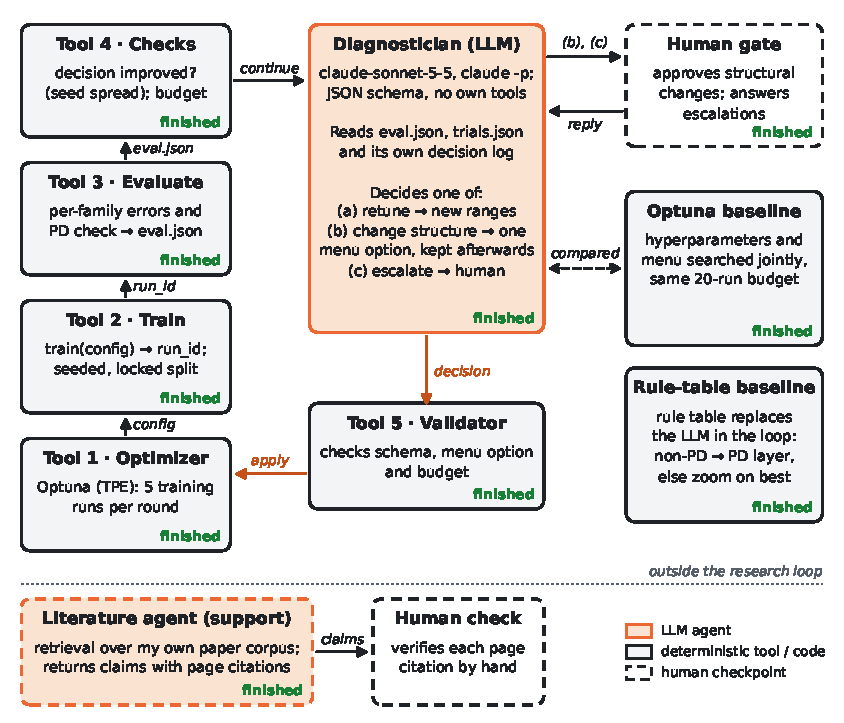
\includegraphics[width=0.74\linewidth]{figures/agent_design_lr3.pdf}
\caption{Research loop and baselines as of Lab Report~3; every module marked \emph{finished} has
run in a full study. Each round, the optimizer launches five training runs, the evaluation tool
writes \texttt{eval.json}, and code judges the previous decision and checks the budget. The
diagnostician's next decision is then validated and applied. Not yet built: the menu options
\texttt{family\_balanced\_loss} and \texttt{physics\_residual}, and the planted-failure harness.
Drawn by \texttt{scripts/make\_design\_figure.py}.}\label{fig:design}
\end{figure}
Figure~\ref{fig:design} shows the loop; the slides linked in C3 give an input and output example
for each finished module.

\subsection*{C2 \quad What changed since Lab Report 2}
\begin{itemize}
\item \textbf{PD output layer (\texttt{pd\_head}).} The three coupling outputs pass through
  partial correlations to a correlation matrix $R = LL^{\mathsf T}$, shrunk as
  $(1-10^{-5})R + 10^{-5}I$, so the normalized compliance block is PD for every input while every
  PD block remains reachable. On the full catalog the labels' smallest block eigenvalue has a
  median of 0.037, and only 4 of 17,222 labels fall below $10^{-4}$, so the margin excludes
  essentially no physical stiffness.
\item \textbf{Validator.} Code rejects a decision whose ranges leave the hard limits, whose menu
  option is not on the menu or is already set, or that exceeds the budget or the cap of three
  structural changes; re-proposing an option that already failed forces an escalation. 37 unit
  tests cover these rules.
\item \textbf{Loop.} One command runs optimize $\to$ evaluate $\to$ check $\to$ agent $\to$
  validate $\to$ gate $\to$ apply. In the studies reported here, the human gate approves every
  structural change unattended, and an escalation stops the study and counts as not solved.
\item \textbf{Rule-table baseline.} A new decider replaces the LLM in the same loop
  (Section~D2).
\end{itemize}

\subsection*{C3 \quad Working loop: the pilot study}
\textbf{Setup.} The pilot ran the full loop on the full catalog: 20 training runs of 100 epochs in
four rounds of five, with \texttt{claude-sonnet-5-5} at high effort deciding after each of the
first three rounds. Each decision was valid on its first call and took 11--13\,s and about
US\$0.07. Table~\ref{tab:pilot} lists the decisions and the verdict that code assigned to each
after the following round.
\begin{table}[!htb]\centering\small
\caption{Agent decisions in the pilot (\texttt{runs/agent-pilot}). A decision counts as
\emph{improved} only if the next round's best run beats the previous best by more than the
seed-to-seed spread (0.01 in loss or 0.04 in non-PD rate).}\label{tab:pilot}
\begin{tabularx}{\linewidth}{@{}lYll@{}}\toprule
After & Decision (agent's reason, condensed) & Best loss & Verdict\\\midrule
Round 0 & change structure: \texttt{pd\_head} on; non-PD 179/2,032, not reduced by retuning &
  0.129 $\to$ 0.119; non-PD 0.088 $\to$ 0 & improved\\
Round 1 & retune: width $\{256, 512\}$, lr $[3\times10^{-4}, 2\times10^{-3}]$, batch $\{32, 64\}$;
  best runs at the top of the width range & 0.119 $\to$ 0.085 & improved\\
Round 2 & retune: layers $[5, 8]$, lr $[2\times10^{-4}, 10^{-3}]$; flagged its evidence as thin &
  0.085 $\to$ 0.077 & failed\\\bottomrule
\end{tabularx}
\end{table}

\textbf{Results.} Against the default model with the PD layer (\texttt{main-full-pd}) on the same
2,032 validation lattices, the pilot's best run lowered the loss from 0.110 to 0.077, the median
modulus error from 28.5\% to 21.0\% and the median coupling error from 0.042 to 0.030, with no
non-PD predictions in either. Before the PD layer existed, I had also asked the agent to predict
its effect; it predicted that the non-PD rate would fall to zero in every family while the
coupling error stayed roughly unchanged, and the subsequent run confirmed both. This comparison
is not, however, against a baseline at equal budget, the best run is the minimum of 20 single-seed
runs and therefore optimistically biased, and most good runs reached their best epoch at 92--100
of 100, so the epoch cap still limits accuracy.

\textbf{Failure case.} The first retune added width 512 to the search and the second kept it.
Four of the five width-512 runs, at learning rates of $4.9\times10^{-4}$ to $9.7\times10^{-4}$,
diverged or trained poorly (three of them in the last round, with losses near 0.82), and the
width-512 runs took 11--20\,h each. Because the budget counts runs rather than compute, the agent
paid nothing for this choice, and it never sees training time. The agent's evidence also
contained two arithmetic slips (for instance, ten remaining runs described as one round of five);
the validator checks the budget itself, but evidence text is not checked.

\textbf{Demo slides.}
\href{https://docs.google.com/presentation/d/1fSxOqZ8NDfNTN7x3azsYzhtkwMNODy9I/edit?usp=sharing}{\nolinkurl{docs.google.com/presentation/d/1fSxOqZ8NDfNTN7x3azsYzhtkwMNODy9I}}.
One slide per finished module gives an input, the output and a failure case, followed by plots of
its outputs and the final comparison of the three conditions.

\section*{D \quad Evaluation}

\subsection*{D1 \quad LLM-free check, as implemented}
Three checks run in code, none of which involves an LLM. First, the evaluation tool tests every
predicted stiffness for positive definiteness through the smallest eigenvalue of the normalized
$3\times3$ compliance block, with a tolerance of $3.6\times10^{-7}$ derived from single-precision
rounding. Second, the validator accepts or rejects each decision before it runs. Third, after the
round that follows a decision, code compares that round's best run with the best run before the
decision and labels the decision \emph{improved} only if the loss falls by more than the
seed-to-seed spread or the non-PD rate falls by more than its spread. On the full catalog, two
seeds of the default model differ by 0.012 in loss without the PD layer and by 0.0035 with it, and
by 0.041 in non-PD rate, which set the thresholds of 0.01 and 0.04. The pilot's last verdict
(a drop of 0.0076) lies inside this spread, so \emph{failed} here means \emph{not
distinguishable from noise}, not \emph{harmful}.
On the 2,000-lattice subset used below, the same two seeds differ by 0.008 in loss without the PD
layer and by 0.023 with it, so the loss threshold there is 0.02; both seeds gave 19 non-PD
predictions among 239 validation lattices, which provides no usable spread, so the non-PD
threshold of 0.04 is carried over from the full catalog.
\textbf{Success.} At equal budget, the agent loop must reach a lower best validation loss than
both baselines by more than the seed spread; the non-PD rate of the final model and the number of
runs to reach the best baseline's loss are secondary measures.

\subsection*{D2 \quad Baselines, run}
All three conditions use the 2,000-lattice subset of the locked split, the same search ranges,
20 training runs of 100 epochs and the same sampler seed. Optuna searches the hyperparameters and
the two menu switches jointly from the first run. The rule table runs in the same loop as the
agent: if the best run has non-PD predictions and the PD layer is off, it enables the layer;
otherwise it narrows each range around the best run so far (a factor of three either side on a
log scale, $\pm1$ layer, the widths of the three best runs), widening rather than repeating a zoom
that already failed. The rule table therefore commits sequentially exactly as the agent does, so
any difference between the two isolates the LLM's diagnosis from the stepwise search, which was
the confound raised in the review of Lab Report~2. For all three conditions the width is capped at
256, because the pilot showed that width 512 is costly and rarely trains well; the cap removes one
costly mistake the agent could otherwise make, which may favour it.

\begin{table}[!htb]\centering\small
\caption{Subset study, 239 validation lattices in unseen families, one study per condition.
Training time is the sum over runs; the agent's excludes one run whose 39.9\,h of wall time was
almost entirely the laptop in standby.}\label{tab:study}
\begin{tabularx}{\linewidth}{@{}lccccc>{\raggedright\arraybackslash}Xr@{}}\toprule
Condition & Loss & Non-PD & Moduli & Coupl. & Runs & Decisions (verdict) & Time\\\midrule
Optuna alone & 0.225 & 0.084 & 54.0\% & 0.081 & 20 & none & 3.6\,h\\
Rule table & 0.218 & 0 & 52.9\% & 0.080 & 20 & PD layer (improved); two retunes (failed, failed) & 2.5\,h\\
Agent & 0.229 & 0 & 56.8\% & 0.085 & 15 & PD layer (improved); retune (failed); escalate & 2.1\,h\\
Default, PD layer & 0.216, 0.239 & 0 & 47.6, 62.0\% & 0.075, 0.078 & 1 each & two seeds, no search & \\\bottomrule
\end{tabularx}
\end{table}
\textbf{Results.} Table~\ref{tab:study} and the comparison slide show the outcome. The success
criterion of D1 is not met: the agent's best loss (0.229) is the highest of the three, and all
three conditions end within the seed spread of the untuned model with the PD layer (0.216 and
0.239), so on this subset no search procedure, with or without an LLM, improved on the default
configuration. Because the sampler seed was shared, the agent and the rule table trained identical
settings in rounds 0 and 1 and made the same first decision; the PD layer removed every non-PD
prediction in both (from 0.092 and 0.088 to 0). Their losses on those identical settings still
differed by up to 0.024, because training on the CPU is not bit-reproducible, which confirms that
differences of this size are noise. The two loops then diverged. The agent shifted the search
toward the corner of its two best runs, gained 0.0025, and at the next decision escalated with
five runs unused, attributing the remaining error to generalization across unseen families, which
no menu option addresses. The rule table's zoom kept the widths of its three best runs, which
admitted width 64, and its second retune found the best run of the study (0.218), a gain of 0.018
that still falls below the 0.02 threshold. Optuna, searching the PD layer jointly, tried it in
six runs, each paired with a small width or a high learning rate, and its best model still
predicts 8\% of the validation stiffnesses as non-PD. The single clear gain in the study, the PD
layer, was therefore found equally by the rule table and by the agent, and the agent's retune and
escalation did not outperform the rule, which is the narrower claim of B1. Its escalation, which
the loop counts as not solved, may nonetheless be the correct reading of a subset whose 239
validation lattices leave little room for tuning to show.

\section*{E \quad Next steps toward integration (Lab Report 4)}
\begin{itemize}
\item \textbf{Planted failures that a single threshold cannot solve.} The three planned failures
  map one-to-one onto the agent's actions, so a three-line script would pass them. I will add
  compound and ambiguous cases, for example a corrupted family together with a poor
  learning-rate range, or non-PD predictions that arise from divergence rather than from the
  output parametrization, and score the rule table on the same cases.
\item \textbf{Compute-aware budget.} Count the budget in CPU-hours rather than in runs, show the
  agent each run's training time, and then lift the width cap.
\item \textbf{Menu.} Implement \texttt{family\_balanced\_loss}, then \texttt{physics\_residual},
  so that the structural menu offers more than one non-trivial choice.
\item \textbf{Repeats and the locked test set.} Three repeats per condition, and one final
  evaluation of each condition's best model on the 64 locked test families.
\item \textbf{Decision consistency.} Ten calls on the same frozen report, counting how often the
  decision changes.
\end{itemize}
Compute remains the main risk: the full-catalog pilot took six days of wall time. The subset makes
the three-way comparison feasible now, and the full catalog will be reserved for the final runs.

\section*{Progress log}
\textbf{Done since Lab Report 2} (\texttt{LOG.md}, 4--15 November): the PD output layer with 22
tests; the decision schema and validator with 37 tests; the diagnostician and its first validated
decision; the loop with human gate, outcome check and thresholds from the seed spread; the
full-catalog pilot; the rule-table baseline and the three-way subset study.
\textbf{Remaining:} the two further menu options, the planted-failure harness, repeats and the
test-set evaluation. \textbf{Bottleneck:} CPU time (E).
\textbf{Maintenance:} seven commits since Lab Report~2 was merged on 1 November
(4--15 November), and \texttt{LOG.md} entries on 4, 5, 11 and 15 November.

\section*{AI usage disclosure}
\textbf{Tools.} Claude Code (\texttt{claude-opus-5-5}) built this project under my direction: it
wrote the code, tests and figure script and drafted this report from \texttt{LOG.md} and the run
folders. The diagnostician itself is \texttt{claude-sonnet-5-5}, called through \texttt{claude -p}
with no tools. The new papers in A2 were found by a Claude Code literature subagent run from
the same session; its notes are in \texttt{literature\_review/lr3/}.
\textbf{My role and checks.} I made the design decisions, including the width cap, the rule-table
baseline and the thresholds, and reviewed each step and each commit. Every number in this report
comes from a logged run in \texttt{runs/} or from \texttt{LOG.md}, and I read every cited paper and
checked each cited section.

\begin{thebibliography}{9}\footnotesize\setlength{\itemsep}{0pt}
\bibitem{lumpe} T.~S. Lumpe, T.~Stankovi\'c. Exploring the property space of periodic cellular
  structures based on crystal networks. \emph{PNAS} 118(7), 2021. doi:10.1073/pnas.2003504118.
\bibitem{ferreira} F.~Ferreira, L.~Wobbe, A.~Krishnakumar, F.~Hutter, A.~Zela. Can LLMs beat
  classical hyperparameter optimization algorithms? A study on autoresearch. arXiv:2603.24647v5,
  2026.
\bibitem{huai} T.~Huai, T.~Fan, X.~Chen, et al. AgentHPOBench: A benchmark for evaluating LLM
  agents as sequential hyperparameter optimizers. arXiv:2607.29626, 2026.
\bibitem{rodrigues} Rodrigues, Vas, DCosta, Prabhakaran. When is an LLM worth it for
  hyperparameter optimization? A budget-matched study on tabular data finds the warm-start is a
  default configuration, not the model. arXiv:2606.21641, 2026.
\bibitem{kim} J.~Kim, N.~Humbatova, G.~Jahangirova, S.~Yoo, P.~Tonella. Fault localisation and
  repair for DL systems: an empirical study with LLMs. arXiv:2506.03396, 2025.
\bibitem{aitm} A.~Rao, N.~K.~Advani. AI Training Manager: bounded closed-loop control of adaptive
  training recipes. arXiv:2606.29871, 2026.
\end{thebibliography}

\end{document}
